\documentclass[a4paper]{report}
\usepackage[utf8]{inputenc}
\usepackage[T1]{fontenc}
\usepackage{textcomp}

\usepackage{url}

\usepackage{hyperref}
\hypersetup{
    colorlinks,
    linkcolor={black},
    citecolor={black},
    urlcolor={blue!80!black}
}

\usepackage{graphicx}
\usepackage{wrapfig}
\usepackage{adjustbox}
\usepackage{float}
\usepackage[usenames,dvipsnames]{xcolor}

\usepackage{listings}

\lstset{
    language=Python,
    basicstyle=\ttfamily\footnotesize,
    keywordstyle=\color{blue},
    stringstyle=\color{red},
    commentstyle=\color{gray},
    showstringspaces=false,
    frame=single,
    numbers=left,
    numberstyle=\tiny,
    breaklines=true,
    tabsize=4
}

% \usepackage{cmbright}

\usepackage{amsmath, amsfonts, mathtools, amsthm, amssymb}
\usepackage{mathrsfs}
\usepackage{cancel}

\newcommand\N{\ensuremath{\mathbb{N}}}
\newcommand\R{\ensuremath{\mathbb{R}}}
\newcommand\Z{\ensuremath{\mathbb{Z}}}
\renewcommand\O{\ensuremath{\emptyset}}
\newcommand\Q{\ensuremath{\mathbb{Q}}}
\newcommand\C{\ensuremath{\mathbb{C}}}
\let\implies\Rightarrow
\let\impliedby\Leftarrow
\let\iff\Leftrightarrow
\let\epsilon\varepsilon

% horizontal rule
\newcommand\hr{
    \noindent\rule[0.5ex]{\linewidth}{0.5pt}
}

\usepackage{tikz}
% \usepackage{tikzmark}
\usepackage{pgfplots}
\usepackage{tikz-cd}

\usetikzlibrary{calc, arrows.meta, positioning, angles, quotes, patterns}

% theorems
\usepackage{thmtools}
\usepackage{thm-restate}
\usepackage[framemethod=TikZ]{mdframed}
\mdfsetup{skipabove=1em,skipbelow=0em, innertopmargin=12pt, innerbottommargin=8pt}

\theoremstyle{definition}

\makeatletter

\declaretheoremstyle[
    headfont=\bfseries\sffamily\color{ForestGreen!70!black}, bodyfont=\normalfont,
    mdframed={
        linewidth=2pt,
        rightline=false, topline=false, bottomline=false,
        linecolor=ForestGreen, backgroundcolor=ForestGreen!5,
    }
]{thmgreenbox}

\declaretheoremstyle[
    headfont=\bfseries\sffamily\color{NavyBlue!70!black}, bodyfont=\normalfont,
    mdframed={
        linewidth=2pt,
        rightline=false, topline=false, bottomline=false,
        linecolor=NavyBlue, backgroundcolor=NavyBlue!5,
    }
]{thmbluebox}

\declaretheoremstyle[
    headfont=\bfseries\sffamily\color{NavyBlue!70!black}, bodyfont=\normalfont,
    mdframed={
        linewidth=2pt,
        rightline=false, topline=false, bottomline=false,
        linecolor=NavyBlue
    }
]{thmblueline}

\declaretheoremstyle[
    headfont=\bfseries\sffamily\color{RawSienna!70!black}, bodyfont=\normalfont,
    mdframed={
        linewidth=2pt,
        rightline=false, topline=false, bottomline=false,
        linecolor=RawSienna, backgroundcolor=RawSienna!5,
    }
]{thmredbox}

\declaretheoremstyle[
    headfont=\bfseries\sffamily\color{RawSienna!70!black}, bodyfont=\normalfont,
    numbered=no,
    mdframed={
        linewidth=2pt,
        rightline=false, topline=false, bottomline=false,
        linecolor=RawSienna, backgroundcolor=RawSienna!1,
    },
    qed=\qedsymbol
]{thmproofbox}

\declaretheoremstyle[
    headfont=\bfseries\sffamily\color{NavyBlue!70!black}, bodyfont=\normalfont,
    numbered=no,
    mdframed={
        linewidth=2pt,
        rightline=false, topline=false, bottomline=false,
        linecolor=NavyBlue, backgroundcolor=NavyBlue!1,
    },
]{thmexplanationbox}

\declaretheorem[numberwithin=chapter, style=thmgreenbox, name=Definition]{definition}
\declaretheorem[sibling=definition, style=thmredbox, name=Corollary]{corollary}
\declaretheorem[sibling=definition, style=thmredbox, name=Proposition]{prop}
\declaretheorem[sibling=definition, style=thmredbox, name=Theorem]{theorem}
\declaretheorem[sibling=definition, style=thmredbox, name=Lemma]{lemma}
\declaretheorem[sibling=definition, style=thmbluebox,  name=Example]{eg}
\declaretheorem[sibling=definition, style=thmbluebox,  name=Nonexample]{noneg}
\declaretheorem[sibling=definition, style=thmblueline, name=Remark]{remark}




\declaretheorem[numbered=no, style=thmexplanationbox, name=Proof]{explanation}
\declaretheorem[numbered=no, style=thmproofbox, name=Proof]{preuve}
\declaretheorem[style=thmbluebox,  numbered=no, name=Exercise]{ex}
\declaretheorem[style=thmblueline, numbered=no, name=Note]{note}

% \renewenvironment{proof}[1][\proofname]{\begin{replacementproof}}{\end{replacementproof}}

% \AtEndEnvironment{eg}{\null\hfill$\diamond$}%

\newtheorem*{uovt}{UOVT}
\newtheorem*{notation}{Notation}
\newtheorem*{previouslyseen}{As previously seen}
\newtheorem*{problem}{Problem}
\newtheorem*{observe}{Observe}
\newtheorem*{property}{Property}
\newtheorem*{intuition}{Intuition}


\declaretheoremstyle[
    headfont=\bfseries\sffamily\color{RawSienna!70!black}, bodyfont=\normalfont,
    mdframed={
        linewidth=2pt,
        rightline=false, topline=false, bottomline=false,
        linecolor=RawSienna, backgroundcolor=RawSienna!5,
    }
]{todo}
\declaretheorem[numbered=no, style=todo, name=TODO]{TODO}


\usepackage{etoolbox}

\AtEndEnvironment{vb}{\null\hfill$\diamond$}%
\AtEndEnvironment{intermezzo}{\null\hfill$\diamond$}%




% http://tex.stackexchange.com/questions/22119/how-can-i-change-the-spacing-before-theorems-with-amsthm
% \def\thm@space@setup{%
%   \thm@preskip=\parskip \thm@postskip=0pt
% }

\usepackage{xifthen}

\def\testdateparts#1{\dateparts#1\relax}
\def\dateparts#1 #2 #3 #4 #5\relax{
    \marginpar{\small\textsf{\mbox{#1 #2 #3 #5}}}
}

\def\@lesson{}%
\newcommand{\lesson}[3]{
    \ifthenelse{\isempty{#3}}{%
        \def\@lesson{Lecture #1}%
    }{%
        \def\@lesson{Lecture #1: #3}%
    }%
    \subsection*{\@lesson}
    \testdateparts{#2}
}

% fancy headers
\usepackage{fancyhdr}
\pagestyle{fancy}

% \fancyhead[LE,RO]{Gilles Castel}
\fancyhead[RO,LE]{\@lesson}
\fancyhead[RE,LO]{}
\fancyfoot[LE,RO]{\thepage}
\fancyfoot[C]{\leftmark}
\renewcommand{\headrulewidth}{0pt}

\makeatother

% figure support (https://castel.dev/post/lecture-notes-2)
\usepackage{import}
\usepackage{xifthen}
\pdfminorversion=7
\usepackage{pdfpages}
\usepackage{transparent}
\usepackage[margin=0.8in]{geometry}
\newcommand{\incfig}[1]{%
    \def\svgwidth{\columnwidth}
    \import{./figures/}{#1.pdf_tex}
}

% %http://tex.stackexchange.com/questions/76273/multiple-pdfs-with-page-group-included-in-a-single-page-warning
\pdfsuppresswarningpagegroup=1
\pgfplotsset{compat=1.11}
\usepackage{subcaption}

\author{Yehor Korotenko}

\newcommand{\scalar}[2]{\langle #1, #2 \rangle}
\newcommand{\scalair}[1]{\left\langle #1 \right\rangle}

% fancy chapters
\usepackage{lipsum}
\usepackage[Lenny]{fncychap}
\ChNameUpperCase
\ChNumVar{\fontsize{40}{42}\usefont{OT1}{ptm}{m}{n}\selectfont}
\ChTitleVar{\Large\sc}



\title{Algebre Linéaire}


\begin{document}
\maketitle
\begin{abstract}
    Le cours parte sur deux sujets liées:
    \begin{enumerate}
        \item la théorie des espaces euclidiens (i.e un espace vectoriel réel muni d'un produit scalaire) et leur endomorphismes
        \item la réduction des endomorphismes d'un espace vectoriel de dimension finie
    \end{enumerate}
\end{abstract}
\section{Notion utiles}
\begin{theorem}
   du rang: Soit une application $f: E \to E'$ avec $E$ et  $E'$ des éspaces vectoriels, alors: 
   \[
        dim(E) = dim(Ker(f)) + dim(Im(f)) 
   \] 
   cela aussi signifie que $Ker(f) \oplus  Im(f) = E$ (image et kernel sont en somme directe). 
\end{theorem}
\begin{intuition}
   Toute application linéaire peut être representée comme une matrice 
\end{intuition}


\chapter{Premier cours}
\section{Éspaces $\R^d$  $\C^d$}
\begin{definition}
    \[
        \R^d = \{ X = (x_1, \ldots, x_d), x_i \in \R\}
    \] 
    $x_1, \ldots, x_d$ coordonnées cartésiennes de X
\end{definition}
\begin{eg}
   $d = 2$ coordonnées polaires:  
   \begin{align*}
      &x = r \cos \theta \\
        & y = r \sin \theta\\
        &0 \le r \le  \infty \quad \theta \in [0, 2\pi[
   \end{align*}
   \begin{center}
       
\begin{tikzpicture}
    % Create the axis
    \begin{axis}[
        axis lines=middle,
        xmin=-1, xmax=3,
        ymin=-1, ymax=3,
        xlabel={$x$},
        ylabel={$y$},
        axis equal,
        height=6cm
    ]
        % Draw the vector
        \addplot[->, thick, blue] coordinates {(0,0) (3,2)} node[right] {$\vec{v}$};

        % Draw x-axis projection manually
        \draw[thick] (axis cs: 0,0) -- (axis cs: 3,0);

        % Use TikZ outside \addplot for \pic
        \node (A) at (2, 0) {};
        \node (C) at ($(0,0)!0.5!(3,2)$) {};
        \node (B) at (0, 0) {};
        \node[above] (_) at ($(0,0)!0.5!(3,2)$) {$r$};
        
        \pic [draw,-, black, angle eccentricity=1.2, angle radius=1cm,"$\theta$"] {angle = A--B--C};
    \end{axis}
\end{tikzpicture}
\end{center}
\end{eg}

\begin{definition}
    $\R^d$ est un espace vectoriel sur  $\R$ 
    \begin{align*}
        &\vec{X} + \vec{Y} = (x_1 + y_1, \ldots, x_d + y_d)\\
        &\lambda X = (\lambda x_1, \ldots, \lambda x_d) \quad \lambda \in \R\\
        &\vec{0}_d = \vec{0} = (0, \ldots, 0)
    \end{align*}
\end{definition}
\begin{definition}\label{def:prod_scalaire}
    Un \textbf{produit scalaire}:
    \[
    X \cdot Y = x_1y_1 + x_2y_2 + \ldots x_dy_d = \|X\|\|Y\|\cos(\theta) \text{ (où } \theta \text{ est une angle entre } X \text{ et } Y \text{)}
    \] 
\end{definition}
\begin{intuition}
    Ce produit nous dit \textit{how closely the vectors point in the same direction} (cosinus tend vers 1 quand $\theta$ tend vers 0º, et cosinus tend vers 0 quand  $\theta$ tend vers 90º). Et ce produit nous permet d'avoir une projection de $X$ sur $Y$ par la formule:
    \[
    Proj(X) = \frac{X \cdot Y}{\|Y\|} \cdot \frac{Y}{\|Y\|}
    \] 
    $X \cdot Y$ donne la longeur de  $X$ et  $Y$ ensemble, en divisant cette longeur par  $\|Y\|$ (la longeur de $Y$) on obtient la longeur de $X$ sur Y, il nous reste de multiplier cette longeur par un vecteur unitaire(de longeur 1) qui pointe dans la même direction que  $Y$, (on l'obtient par $\frac{Y}{\|Y\|}$)
   \begin{center}
      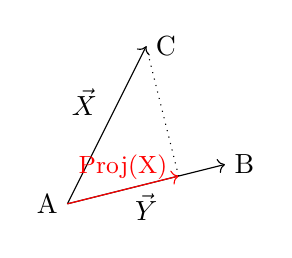
\begin{tikzpicture}
         \coordinate (A) at (0, 0); 
         \coordinate (B) at (2, 0.5);
         \coordinate (C) at (1, 2);
         \coordinate (newB) at (1.4117647059, 0.3529411765);
         \coordinate (dotBC) at (2, 1);
         \node[left] (_) at (A){A};
         \node[right] (_) at (B){B};
         \node[right] (_) at (C){C};
         \draw[->] (A) -- (B);
         \node[above left] (...) at ($(A)!0.5!(C)$) {$\vec{X}$};
         \node[below] (...) at ($(A)!0.5!(B)$) {$\vec{Y}$};
         \draw[->] (A) -- (C);
         \draw[->, red, thin] (A) -- (newB);
         \draw[dotted] (C) -- (newB);
         \node[above, red] (_) at ($(A)!0.5!(newB)$){\small Proj(X)};
      \end{tikzpicture} 
   \end{center}
\end{intuition}
\begin{prop}
    Produit scalaire respectes ces propriétés:
    \begin{enumerate}
        \item bilinaiarité $\quad \lambda \in \R$
            \begin{enumerate}
                \item $(X + Y) \cdot Z = X \cdot Z + Y \cdot Z$
                \item $(\lambda X) \cdot Z = \lambda (X \cdot Z)$
                \item $Z \cdot (X + Y) = Z \cdot X + Z \cdot Y$ 
                \item $Z \cdot (\lambda X) = \lambda (Z \cdot X)$
            \end{enumerate}
        \item symétrie $X \cdot Y = Y \cdot X$
        \item défini positif:  $X \cdot X \ge 0$ et $X \cdot X = 0 \iff X = 0_d$
    \end{enumerate}
\end{prop}
\begin{prop}
    \underline{Cauchy-Schwarz}:\\ 
    \[
        |X \cdot Y| \le (X \cdot X)^{\frac{1}{2}}(Y \cdot Y)^{\frac{1}{2}}
    \] 
\end{prop}
\begin{definition}\label{def:norm_eucl}
    La \textbf{norme euclidienne} d'un vecteur $X$ est noté:
   \[
       \|X\| = \left(\sum_{n=1}^{d} x_i^2\right)^{\frac{1}{2}} = \sqrt{x_1^2 + \ldots + x_d^2} = (X \cdot X)^{\frac{1}{2}}
   \] 
   souvent noté $\|X\|_2$
\end{definition}
\begin{intuition}
   Par le théorème de Pythogore, c'est une longeur de ce vecteur. 
\end{intuition}
\begin{prop}
    La norme suit ces propriétés:
   \begin{enumerate}
       \item $\|\lambda X\| = |\lambda|\|X\| \, X \in \R^d, \, \lambda \in \R$
       \item $\|X + Y\| \le \|X\| + \|Y\| \text{ (inégalité triangulaire)}$
       \item $\|X\| \ge 0$ et $\|X\| = 0 \iff X = 0_d$
   \end{enumerate}
\end{prop}
\begin{explanation}
    de (2)
    \begin{align*}
        \|X + Y\|^2 &= (X + Y)\cdot(X + Y) = X \cdot (X + Y) + Y \cdot (X + Y) = X \cdot X + X \cdot Y + Y \cdot X + Y \cdot Y\\
                    &= \|X\|^2 + 2X \cdot Y + \|Y\|^2 \le \|X\|^2 + 2\|X\| \|Y\| + \|Y\|^2 = (\|X\| + \|Y\|)^2
    \end{align*}
\end{explanation}
\begin{definition}
    Une \underline{norme} sur $\R^d$ est une application  $N: \: \R^d \to \R$ tell que:
    \begin{enumerate}
        \item $N(\lambda X) = |\lambda|N(X)$
        \item  $N(X + Y) \le N(X) + N(Y)$
        \item $N(X) \ge 0$ et $N(X) = 0 \iff X = 0_d$
    \end{enumerate}
\end{definition}
\begin{eg}
   \begin{align*}
       &\|X\|_1 = \sum_{n=1}^{d} |x_i|\\
       &\|X\|_{\infty} = \underset{1\le i \le n}{max} |x_i|
   \end{align*} 
\end{eg}
\section{Éspace $\C^d$}
\begin{definition}
    \[
        \C^d = \{ X = (x_1, \ldots, x_d): \: x_i \in \C\}
    \] 
    \begin{align*}
    &z \in \C \quad \overline{z} = a - ib \quad \overline{z}z = a^2 + b^2 \quad |z| = \sqrt{\overline{z}z} = \sqrt{a^2 + b^2}  \\
    &z = a + ib \qquad a = Re\,z,\,b = Im\,z\\
    &Re\,X = (Re\,x_1, \ldots, Re\,x_d) \in \R^d\\
    &Im\,X = (Im\,x_1, \ldots, Im\,x_d) \in \R^d\\
    &\underset{\in \C^d}{X} = \underset{\in \R^d}{Re\,X} + i\underset{\in \R^d}{\:Im\,X}\\
    \end{align*}
    $\C^d$ est un espace vécrotiel sur  $\C$ (même formules avec $\lambda \in \C$ corps des scalaires)
\end{definition}
\begin{definition}
    \underline{Produit scalaire:}
    \[
        (X|Y) = \sum_{n=1}^{d} \overline{x_i}y_i \in \C
    \] 
\end{definition}
\begin{prop}
   . 
   \begin{enumerate}
       \item $(X|Y)$ est "linéaire par rapport à Y"
           \begin{itemize}
               \item $(Z|X + Y) = (Z|X) + (Z|Y)$
               \item $(Z|\lambda X) = \lambda(Z|X) \quad \lambda \in \C$
               \item  $(Z|\lambda X + \mu Y) = \lambda(Z|X) + \mu(Z|Y)$
               \item  $(X + Y|Z) = (X|Z) + (Y|Z)$
               \item $(\lambda X|Z) = \overline{\lambda}(X|Z) \quad \lambda \in \C$
               \item $(\lambda X + \mu Y|Z) = \overline{\lambda}(X|Z) + \mu(Y|Z)$
           \end{itemize}
       \item $(Y|X) = \overline{(X|Y)}$
       \item $(X|X) = \sum_{n=1}^{d} \overline{x_i}x_i = \sum_{n=1}^{d} |x_i|^2$\\
           $(X|X) \ge 0$ et $(X|X) = 0 \iff X = 0_d$
   \end{enumerate}
\end{prop}
\begin{explanation}
    On a Cauchy-Schwarz:
    \begin{align*}
        (X|Y) \le (X|X)^{\frac{1}{2}}(Y|Y)^{\frac{1}{2}}
    \end{align*}
    même preuve qu'avant
\end{explanation}
On pose:
\begin{align*}
    \|X\| & \text{(ou }\|X\|_2\text{)}\\
          &= (X|X)^{\frac{1}{2}} = \left( \sum_{n=1}^{d} |x_i|^2 \right)^2
\end{align*}
norme hibertienne
\[
    \underset{\in \C^d}{\|X\|^2} = \underset{\in \R^d}{\|Re\,X\|^2} + i\underset{\in \R^d}{\:\|Im\,X\|^2}\\
\] 
\begin{lemma}
   \begin{align*}
       \|X\| = \underset{\|Y\|\le 1}{sup|(X|Y)|}
   \end{align*} 
\end{lemma}
\begin{explanation}
    $|(X|Y)| \le \|X\|\|Y\| \le \|X\|$ si $\|Y\| \le 1$
    \[
    \underset{\|Y\|\le 1}{sup|(X|Y)|}
    \] 
    \underline{Autre sens:} 
    \begin{align*}
        &X \neq 0 \quad Y =  \frac{X}{\|X\|} = \lambda X \quad \lambda = \frac{1}{\|X\|}\\
        &\|Y\| = |\lambda|\|X\| = \frac{1}{\|X\|}\|X\| = 1\\
        &(X|Y) = (X|\frac{X}{\|X\|}) = \frac{1}{\|X\|}(X|X) = \|X\|\\
        &sup \{|(X|Y)|: \, \|Y\| \le  1\}\\
        &\|X\| \le sup \{|(X|Y)|: \, \|Y\|\le 1\} \quad \text{(prendre }Y = \frac{X}{\|X\|}\text{)}
    \end{align*}

\end{explanation}
\underline{Autres normes sur $\C^d$}
\begin{itemize}
    \item $\|X\|_1 = \sum_{n=1}^{d} |x_i| \quad X \in \C^d$
    \item $\|X\|_{\infty} = \underset{1\le i \le d}{sup} |x_i|$
\end{itemize}
\section{Distance sur $\R^d$}
On oublie norme et produit scalaire. On introduit la distance
\begin{definition}\label{def:distance} La distance
    \[
        d(X, Y) = \|X - Y\| 
    \] 
\end{definition}
\begin{definition} La distance euclidienne
    \[
        d(X, Y) = \|X - Y\| = \sqrt{\sum_{n=1}^{d} (x_i - y_i)^2} 
    \] 
\end{definition}
\begin{prop}
    \begin{align*}
        d: \R^d &\longrightarrow \R \\
        (X, Y) &\longmapsto d((X, Y)) 
    .\end{align*}
    \begin{enumerate}
        \item $d(X, Y) = d(Y, X)$ (symétrie)
        \item $d(X, Y) \le d(X, Z) + d(Z, Y)$ (inég. triangulaire) $\forall X, Y, Z$ 
        \item $d(X, Y) \ge 0 \quad \forall X, Y$ et $d(X, Y) = 0 \iff X = Y$ 
    \end{enumerate}
\end{prop}
\begin{eg} Distances
   \begin{enumerate}
       \item $d_2(X, Y) = \|X - Y\|_2$ (distance euclidienne sur $\R^d$)
       \item $d_1(X, Y) = \|X - Y\|_1$\\
           $d_{\infty}(X, Y) = \|X - Y\|_{\infty}$
       \item distance logarithmique sur $\R_+$:  $d(a, b) = |b - a|$
           \[
               \log_{10}(a) = \frac{\log(a)}{\log(10)}
           \] 
           $x, y \in ]0, +\infty[$\\ 
           $d_{\log}(x, y) = |\log_{10}(\frac{y}{x})|$ \\
           $i$ est une distance sur  $]0, +\infty[$\\
           $d_{\log}(100, 110) = \log_{10}(1,1)$
       \item distance SNCF
           \begin{center}
               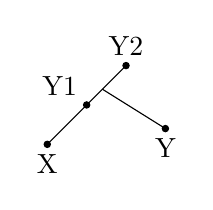
\begin{tikzpicture}
                  \coordinate (X) at (0, 0); 
                  \coordinate (Y) at (1.5, 0.2);
                  \coordinate (Y2) at (1, 1);
                  \coordinate (Y1) at ($(X)!0.5!(Y2)$);
                  \draw (X)--(Y2);
                  \draw (Y)--($(X)!0.7!(Y2)$);
                  \draw[fill=black] (X) circle (0.4mm);
                  \draw[fill=black] (Y) circle (0.4mm);
                  \draw[fill=black] (Y2) circle (0.4mm);
                  \draw[fill=black] (Y1) circle (0.4mm);
                  \node[below] (_) at (X){X};
                  \node[below] (_) at (Y){Y};
                  \node[above left] (_) at (Y1){Y1};
                  \node[above] (_) at (Y2){Y2};
               \end{tikzpicture}
               
           \end{center}
           $d(X, Y)$ distance usuelle dans  $\R^2$
           on pose:
            \begin{align*}
               \delta(X, Y) = \begin{cases}
                   d(X, Y) \text{ si } X, 0, Y \text{ alignés}\\
                   d(X, 0) + d(0, Y) \text{ sinon }
               \end{cases}
           \end{align*}
   \end{enumerate}
\end{eg}
\chapter{Éspaces métriques}
\begin{definition}
    $E$ muni d'une application de distance $d$ (voir Definition \ref{def:distance}) se note  $(E, d)$: \underline{espace métrique}
\end{definition}
\begin{remark}
   si $d_1 \neq d_2$ $(E, d_1)$ n'a rien à faire avec  $(E, d_2)$ 
\end{remark}
\begin{remark}
    Retenir la version suivante de l'inégalité triangulaire:
    \[
        |d(x, z) - d(y, z)| \le d(x, y)
    \] 
\end{remark}
\begin{remark}
    \underline{Distance induite:}\\
    Si $(E, d)$ espace métrique et  $U \subset E$. Je peux restreidnre $d$ à  $U \times U$:  $(U, d)$ est aussi un éspace metrique.
\end{remark}
\section{Boules dans un espace métrique}
\begin{definition}
    $(E, d)$ espace métrique. Soit  $x_0 \in E$ et $r \ge  0$
    \begin{enumerate}
        \item $B(x_0, r) = \{ x \in E: d(x_0, x) < r$ \} boule ouverte de centre $x_0$, de rayon $r$
        \item $B_f(x_0, r) = \{ x \in E: d(x_0, x) \le  r$\} boule fermée de centre $x_0$, de rayon $r$
    \end{enumerate}
\end{definition}
\begin{figure}
    \centering
    \begin{subfigure}{0.45\textwidth}
        \centering
        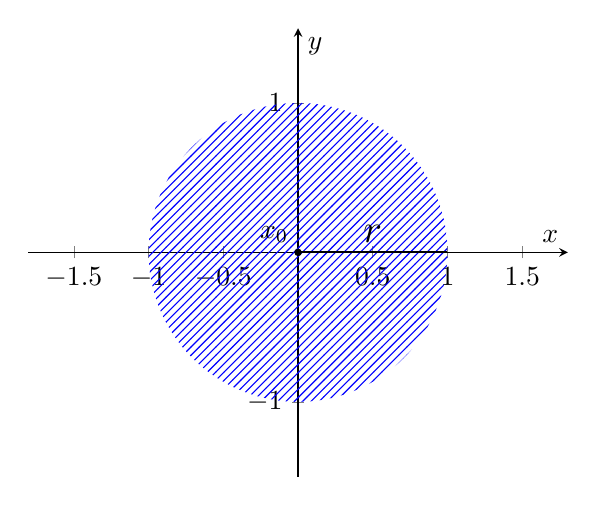
\begin{tikzpicture}
            \begin{axis}[
                axis equal, % Ensures the circle appears round
                axis lines=middle,
                xlabel={$x$},
                ylabel={$y$},
                xmin=-1.5, xmax=1.5,
                ymin=-1.5, ymax=1.5
                ]
                % Plot a circle with radius 1
                \addplot [
                    domain=0:360,       % Angle range
                    samples=200,        % Smoothness
                    fill=none,          % No solid fill color
                    pattern=north east lines, % Hatch pattern
                    pattern color=blue,
                    draw=none           % No outline
                    ] ({cos(x)}, {sin(x)}); 
                \node[above left] (_) at (0, 0){$x_0$};
                \draw[fill=black] (0, 0) circle (0.4mm);
                \draw[thick] (0,0)--(1,0);
                \node[above] (r) at ($(0,0)!0.5!(1,0)$){\Large$r$};
            \end{axis}
        \end{tikzpicture}
        \caption{boules ouverte (i.e $d(x_0, x) < r$)}
    \end{subfigure}
    \hfill
    \centering
    \begin{subfigure}{0.45\textwidth}
        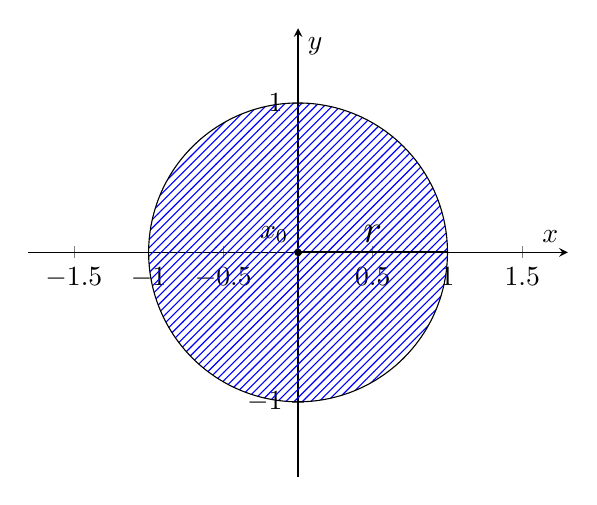
\begin{tikzpicture}
            \begin{axis}[
                axis equal, % Ensures the circle appears round
                axis lines=middle,
                xlabel={$x$},
                ylabel={$y$},
                xmin=-1.5, xmax=1.5,
                ymin=-1.5, ymax=1.5
                ]
                % Plot a circle with radius 1
                \addplot [
                    domain=0:360,       % Angle range
                    samples=200,        % Smoothness
                    fill=none,          % No solid fill color
                    pattern=north east lines, % Hatch pattern
                    pattern color=blue,
                    ] ({cos(x)}, {sin(x)}); 
                \node[above left] (_) at (0, 0){$x_0$};
                \draw[fill=black] (0, 0) circle (0.4mm);
                \draw[thick] (0,0)--(1,0);
                \node[above] (r) at ($(0,0)!0.5!(1,0)$){\Large$r$};
            \end{axis}
        \end{tikzpicture}
        \caption{boules fermée (i.e $d(x_0, x) \le r$)}
    \end{subfigure}
\end{figure}
\begin{lemma}.
   \begin{enumerate}
       \item $B(x_0, 0) = \O$ (car impossible d'avoir des points qui en distance sont strictement plus petit que 0)
       \item $B_f(x_0, 0) = \{x_0\}$
       \item $B(x_0, r_1) \subset B_f(x_0, r_1) \subset B(x_0, r_2)$ si $r_1 < r_2$
       \item $B(x_1, r_1) \subset B(x_0, r)$ si  $d(x_0, x_1) + r_1 \le r$
   \end{enumerate} 
   pic 5
\end{lemma}
\begin{explanation}
   Je suppose que $d(x_0, x_1) \le r$\\ 
   Soit $x \in B(x_1, r_1)$ donc $d(x_1, x) < r_1$ à montrer: $x \in B(x_0, r)$ (i.e $d(x_0, x) < r$?)\\
   L'inégalité triangulaire me dit:
   \begin{align*}
       d(x_0, x) &\le d(x_0, x_1) + d(x_1, x)\\
                 &< d(x_0, x_1) + r_1 \le r\\
                 &\implies x \in B(x_0, r)
   \end{align*}
\end{explanation}

\end{document}
